\documentclass[../main/main.tex]{subfiles}

\newdate{date}{09}{11}{2020}

% \begin{figure}[h!]
% \centering
% \includegraphics[page=6,width=0.8\textwidth]{../lessons/pdf_file/15_lecture.pdf}
% \end{figure}

%\displaydate{date}. Compiled:  \today. Alice.

\begin{document}

\pagestyle{plain}

\section{Lecture 15}


\subsubsection*{Slide 1}

\begin{minipage}[]{0.5\linewidth}
\centering
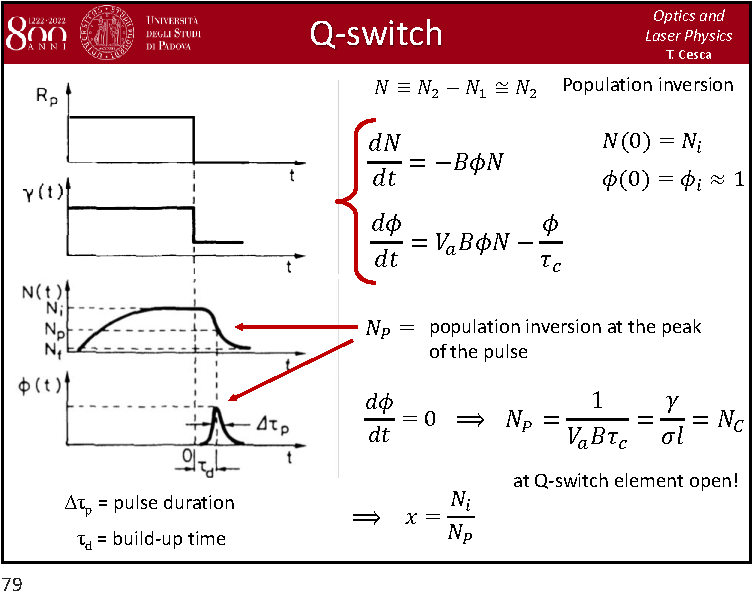
\includegraphics[page=1,width=1\textwidth]{../lessons/pdf_file/15_lecture.pdf}
\end{minipage}
\hspace{0.3cm}\vspace{0.3cm}
\begin{minipage}[c]{0.47\linewidth}

When there is no laser action, the energy is accumulated in the medium as population inversion. The Q-switch idea is to switch the Q factor. We obtain the production with a very high number of photons at the peak.

As already said, we will assume an active Q-switch, hence we have a shutter and we are able to open and close it actively by the outside.
Moreover, the transition between high losses to low losses is assumed to be instaneous. Moreover, we have a pulse pumping.

The other hypothesis are the same for the CW behavior: the population inversion correspond to the population of the upper laser laser and homogeneous energy distribution in the active medium. We have a single mode and homogeneous broadening.

\end{minipage}

We have written the two main rate equations. The timeframe that we willl consider is short enough that we can neglect the in the evolution of the population any contribution related to the pumping. We are simplified the description more assuming that we shut down the pumping. The lifetime of the upper laser level should be sufficiently long in order to be able to accumulate enough initial population inversion. Moreover, there is at least one photon to trigger laser action.

We want to compute the \textbf{population inversion at the peak of the pulse}. To calculate it we can solve this equation when \( \dv{\Phi }{t} = 0  \) (at the peak). It is equal to the critical population inversion when the Q-switch element is open! These values of \( \gamma   \) are after the opening of the Q-switch.

In this case, we can introduce the \textbf{over-treshold factor}: the ratio between the initial population inversion at \( t=0 \) divided by the population inversion at the peak of the pulse. It tells us how much energy we could accumulate in the active medium before making the Q-switch.

\subsubsection*{Slide 2}

\begin{minipage}[]{0.5\linewidth}
\centering
\includegraphics[page=2,width=1\textwidth]{../lessons/pdf_file/15_lecture.pdf}
\end{minipage}
\hspace{0.3cm}\vspace{0.3cm}
\begin{minipage}[c]{0.47\linewidth}

We can compute the \textbf{peak power of the output pulse}. The output power as said is related to the number of photons that we can extract and the number of photons in the cavity. This is the very same expression that we calculated for CW mode. We need to now what is the number of photons at the peak of the pulse to compute the peak power.

We need to callculate \( \Phi_p \) and for doing it we should manipulate the rate equations.

\end{minipage}

\subsubsection*{Slide 3}

\begin{minipage}[]{0.5\linewidth}
\centering
\includegraphics[page=3,width=1\textwidth]{../lessons/pdf_file/15_lecture.pdf}
\end{minipage}
\hspace{0.3cm}\vspace{0.3cm}
\begin{minipage}[c]{0.47\linewidth}

The change \( \dv{\Phi }{N}  \) is this one. If we intregrate both terms of this equations, we have that the difference between \( \Phi - \Phi _i \) (where \( \Phi _i \) is the initial number of photons) is given by the formula. We remember that the initial number of photons is assumed to be equal to one.

But, operating the laser in Q-switch mode we will get that the number of photons at the peak of the pulse can be extremely high, we can reasonably neglect the single extra photon.

\end{minipage}


\subsubsection*{Slide 4}

\begin{minipage}[]{0.5\linewidth}
\centering
\includegraphics[page=4,width=1\textwidth]{../lessons/pdf_file/15_lecture.pdf}
\end{minipage}
\hspace{0.3cm}\vspace{0.3cm}
\begin{minipage}[c]{0.47\linewidth}

We can determine the peak photon number by substituting in the last expression the peak population inversion \( N_p \).

\end{minipage}

\subsubsection*{Slide 5}

\begin{minipage}[]{0.5\linewidth}
\centering
\includegraphics[page=5,width=1\textwidth]{../lessons/pdf_file/15_lecture.pdf}
\end{minipage}
\hspace{0.3cm}\vspace{0.3cm}
\begin{minipage}[c]{0.47\linewidth}

We can write the peak power.

\end{minipage}

\subsubsection*{Slide 6}

\begin{minipage}[]{0.5\linewidth}
\centering
\includegraphics[page=6,width=1\textwidth]{../lessons/pdf_file/15_lecture.pdf}
\end{minipage}
\hspace{0.3cm}\vspace{0.3cm}
\begin{minipage}[c]{0.47\linewidth}

We can calculate the energy of the pulse by the integral in time of the power.
This is in practice the integral of this area of the graph.

This difference \( \Phi (\infty ) - \Phi (0) \) can be assumed equal to zero.

\end{minipage}


\subsubsection*{Slide 7}

\begin{minipage}[]{0.5\linewidth}
\centering
\includegraphics[page=7,width=1\textwidth]{../lessons/pdf_file/15_lecture.pdf}
\end{minipage}
\hspace{0.3cm}\vspace{0.3cm}
\begin{minipage}[c]{0.47\linewidth}

To calculate this integral, we integrate both term in the first rate equation. This is equal to the remaining population inversion at the end and at the beginning.

\end{minipage}

\subsubsection*{Slide 8}

\begin{minipage}[]{0.5\linewidth}
\centering
\includegraphics[page=8,width=1\textwidth]{../lessons/pdf_file/15_lecture.pdf}
\end{minipage}
\hspace{0.3cm}\vspace{0.3cm}
\begin{minipage}[c]{0.47\linewidth}

So, the energy of the pulse is given by the available inversion in order to produce the photons when the pulse is forming, then if we multiply it by the volume of the mode on the active medium we obtain the number of photons produced whitin the pulse. Then, we multiply this by the energy and we get the energy associated to the photon that we have produced. Then, we have to consider only the energy that is extracted.

\end{minipage}

\subsubsection*{Slide 9}

\begin{minipage}[]{0.5\linewidth}
\centering
\includegraphics[page=9,width=1\textwidth]{../lessons/pdf_file/15_lecture.pdf}
\end{minipage}
\hspace{0.3cm}\vspace{0.3cm}
\begin{minipage}[c]{0.47\linewidth}

We need to determine \( N_f \) to calculate \( E \). We can rewrite the number of photons for the final population inversion \( N_f \).

\end{minipage}

\subsubsection*{Slide 10}

\begin{minipage}[]{0.5\linewidth}
\centering
\includegraphics[page=10,width=1\textwidth]{../lessons/pdf_file/15_lecture.pdf}
\end{minipage}
\hspace{0.3cm}\vspace{0.3cm}
\begin{minipage}[c]{0.47\linewidth}

We can simply rewrite the expression.

\( \eta _E \) tells us how much of the initial population inversion is used to produce the pulse of photons when the laser is operating in Q-switch mode and it is called \textbf{inversion (energy)-utilization factor}.
So the smaller is the final population inversion, the larger is the utilization factor. Which fraction of the initial population inversion we are using.

\end{minipage}

\subsubsection*{Slide 11}

\begin{minipage}[]{0.5\linewidth}
\centering
\includegraphics[page=11,width=1\textwidth]{../lessons/pdf_file/15_lecture.pdf}
\end{minipage}
\hspace{0.3cm}\vspace{0.3cm}
\begin{minipage}[c]{0.47\linewidth}

The simplest way to solve this implicit expression is to solve it graphically. This graph relates the inversion utilization factor as a function of the over-threshold factor.

\end{minipage}

\subsubsection*{Slide 12}

\begin{minipage}[]{0.5\linewidth}
\centering
\includegraphics[page=12,width=1\textwidth]{../lessons/pdf_file/15_lecture.pdf}
\end{minipage}
\hspace{0.3cm}\vspace{0.3cm}
\begin{minipage}[c]{0.47\linewidth}

The energy is given by this expression which can be manipulated.

\end{minipage}

\subsubsection*{Slide 13}

\begin{minipage}[]{0.5\linewidth}
\centering
\includegraphics[page=13,width=1\textwidth]{../lessons/pdf_file/15_lecture.pdf}
\end{minipage}
\hspace{0.3cm}\vspace{0.3cm}
\begin{minipage}[c]{0.47\linewidth}

It is possible to make a rough estimation of the \textbf{pulse duration}. That is a very rough way since we are not considering the temporal shape of the pulse, it is like we are considering a square shape of the pulse. However, in this way we can obtain the order of magnitude.

The pulse duration is proportional to the lifetime of a photon in the cavity. Let us stress again that we are considering the condition in which the losses in the cavity are low and the Q-switch is open!

Pulse duration is of the order of magnitude of the photon in the cavity and so it is few nanoseconds.

\end{minipage}

\subsubsection*{Slide 14}

\begin{minipage}[]{0.5\linewidth}
\centering
\includegraphics[page=14,width=1\textwidth]{../lessons/pdf_file/15_lecture.pdf}
\end{minipage}
\hspace{0.3cm}\vspace{0.3cm}
\begin{minipage}[c]{0.47\linewidth}

Another quantity is the \textbf{build-up time}: it represent the time that it takes to the pulse of photons to increase. After the build-up time we have a number of photon in the cavity significantly different from zero.

Typically, we can assume that the build-up time is the moment which is necessary to get a number of photon in the cavity which is 1/10 to the peak value that we get. However, there are no huge differences in how we define this factor and let us take 1/10.

During this time (up to the build-up time), we can assume that the population inversion does not change too much. Assuming this, we can take the second rate equation. We place \( N_i \) instead of \( N_P \).

\end{minipage}

\subsubsection*{Slide 15}

\begin{minipage}[]{0.5\linewidth}
\centering
\includegraphics[page=15,width=1\textwidth]{../lessons/pdf_file/15_lecture.pdf}
\end{minipage}
\hspace{0.3cm}\vspace{0.3cm}
\begin{minipage}[c]{0.47\linewidth}

We integrate that rate equation and we obtain an exponential trend of the number of photons during the build-up time.

Also the build-up time is proportional to the lifetime of a photon in the cavity.

So, after the Q-switch, the timescale that we have to consider is always related to the lifetime of photons in the cavity.

Before \( t=0 \) (before the Q-switch), when the losses were high, the timescale was controlled by the total lifetime of the upper laser level.

\end{minipage}

\subsubsection*{Slide 16}

\begin{minipage}[]{0.5\linewidth}
\centering
\includegraphics[page=16,width=1\textwidth]{../lessons/pdf_file/15_lecture.pdf}
\end{minipage}
\hspace{0.3cm}\vspace{0.3cm}
\begin{minipage}[c]{0.47\linewidth}

Let us substitute \( \Phi _p \) in the expression of the build-up time. This peak value is very high it does not make so much difference to consider a factor 1/10 or 1/20 numerically.

The order of magnitude of the build-up is still some times the lifetime of photons in the cavity.

\end{minipage}

We have calculated all the quantity related to the laser in Q-switch mode. We will compare these with real system to see how close we are to the real number in real systems.



\end{document}
